\section{Orientierung}
Bei der Orientierung auf dem Campus Riedberg geraten Studentenaus allen Semestern und Fachrichtungen regelmä\ss ig in Verzweiflung. Wo finde ich denn Raum \_ \_.111? Wie hei\ss t denn der gro\ss e Hörsaal?\\
Auf dem Riedberg gibt es mehere universtäre Gebäude, das gro\ss e, überaus hübsche, graue ist die Chemie, direkt daneben findet man die Unterkunft von Pharmazie und Biochemie. Dort findet sich auch die Mensa (das wichtigste in diesem Gebäude). Weiter in Richtung der U3 findet man ein gro\ss es rotes Gebäude: die neue Biologie. Au\ss erdem existiern zwei Backsteingebäude: In dem kleineren der beiden sind die Geowissenschaften beheimatet und das grö\ss ere ist das wichtigste für euch: Die Physik. Schräg gegenüber der Physik in Richtung der U8/U9 befindet sich das Infrastrukturzentrum mit Hörsäälen und der Bibliothek.
\vfil
\begin{figure}[h]
	\centering
    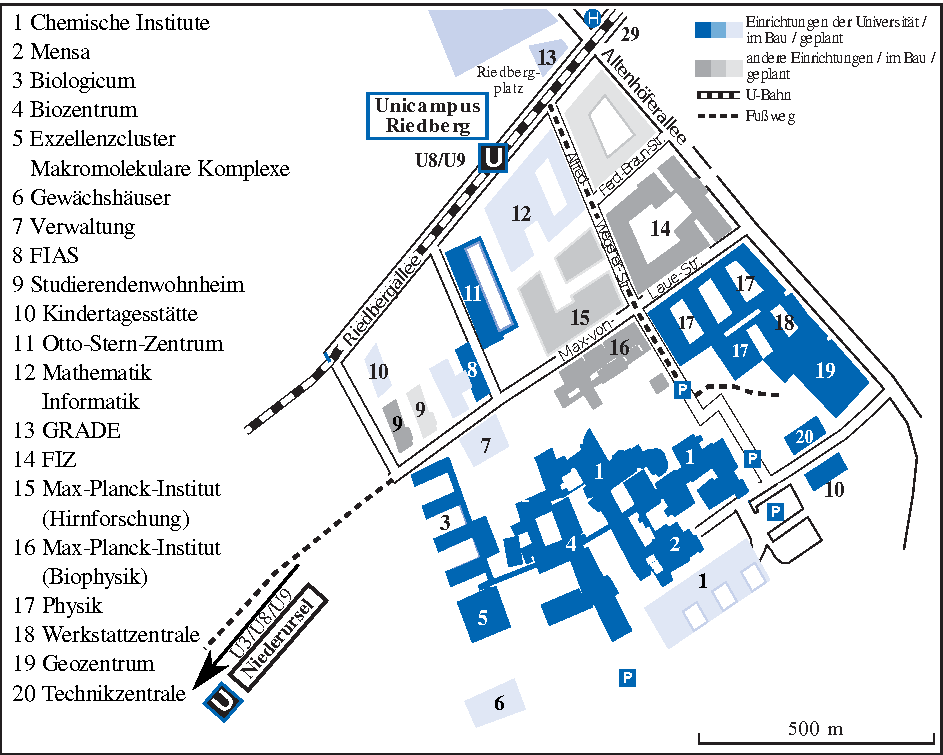
\includegraphics[width=0.80\textwidth]{\imgdir/riedberg-lageplan0.pdf}
\end{figure}
\newpage
Um euch eine komplette Beschreibung des Campus zu liefern, ist dieses Heft zu klein. Daher beschränke ich mich auf die Physik: Der Ort, an dem ihr die meiste Zeit eures Studiums lernen und arbeiten werdet.\\
Die Numerierung der Räume in unserem Gebäude ist zwar logisch, sorgt allerdings immer wieder für Verwirrungen. Jede Raumnummer besteht aus vier bis fünf Zahlen, wobei die hintern drei durch einen Punkt von den restlichen getrennt werden. Vor dem Punkt steht das Stockwerk. Das Erdgeschoss erhhält nicht wie zu erwarten eine 0 oder gar keine Bezeichnung, sondern zwei Unterstriche. Das Untergeschoss erkennt man an einem Unterstrich und einer 0 vor dem Punkt. Die anderen Stockwerke sind standartmä\ss ig bezeichnet (erster Stock: 1; zweiter Stock: 2). Die erste Zahl nach dem Punkt gibt das Gebäude an, die letzten beiden sind einfach die Raumnummer. Welches Gebäude welche Nummer hat, könnt ihr auf unserem Plan sehen.\\
Wenn man jetzt also den Raum \_ \_.208 sucht, dann muss man im Erdgeschoss in das zweite Gebäude gehen (beim Pförtner) und dort am Ende des Ganges findet man dann den Raum (das ist übrigens die Fachschaft).
\vfil
\begin{center}
    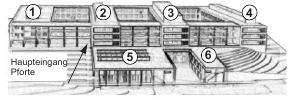
\includegraphics[width=1.00\textwidth]{\imgdir/plan.png}
\end{center}